
%% bare_jrnl_compsoc.tex
%% V1.4
%% 2012/12/27
%% by Michael Shell
%% See:
%% http://www.michaelshell.org/
%% for current contact information.
%%
%% This is a skeleton file demonstrating the use of IEEEtran.cls
%% (requires IEEEtran.cls version 1.8 or later) with an IEEE Computer
%% Society journal paper.
%%
%% Support sites:
%% http://www.michaelshell.org/tex/ieeetran/
%% http://www.ctan.org/tex-archive/macros/latex/contrib/IEEEtran/
%% and
%% http://www.ieee.org/

%%*************************************************************************
%% Legal Notice:
%% This code is offered as-is without any warranty either expressed or
%% implied; without even the implied warranty of MERCHANTABILITY or
%% FITNESS FOR A PARTICULAR PURPOSE! 
%% User assumes all risk.
%% In no event shall IEEE or any contributor to this code be liable for
%% any damages or losses, including, but not limited to, incidental,
%% consequential, or any other damages, resulting from the use or misuse
%% of any information contained here.
%%
%% All comments are the opinions of their respective authors and are not
%% necessarily endorsed by the IEEE.
%%
%% This work is distributed under the LaTeX Project Public License (LPPL)
%% ( http://www.latex-project.org/ ) version 1.3, and may be freely used,
%% distributed and modified. A copy of the LPPL, version 1.3, is included
%% in the base LaTeX documentation of all distributions of LaTeX released
%% 2003/12/01 or later.
%% Retain all contribution notices and credits.
%% ** Modified files should be clearly indicated as such, including  **
%% ** renaming them and changing author support contact information. **
%%
%% File list of work: IEEEtran.cls, IEEEtran_HOWTO.pdf, bare_adv.tex,
%%                    bare_conf.tex, bare_jrnl.tex, bare_jrnl_compsoc.tex,
%%                    bare_jrnl_transmag.tex
%%*************************************************************************

% *** Authors should verify (and, if needed, correct) their LaTeX system  ***
% *** with the testflow diagnostic prior to trusting their LaTeX platform ***
% *** with production work. IEEE's font choices can trigger bugs that do  ***
% *** not appear when using other class files.                            ***
% The testflow support page is at:
% http://www.michaelshell.org/tex/testflow/




% Note that the a4paper option is mainly intended so that authors in
% countries using A4 can easily print to A4 and see how their papers will
% look in print - the typesetting of the document will not typically be
% affected with changes in paper size (but the bottom and side margins will).
% Use the testflow package mentioned above to verify correct handling of
% both paper sizes by the user's LaTeX system.
%
% Also note that the "draftcls" or "draftclsnofoot", not "draft", option
% should be used if it is desired that the figures are to be displayed in
% draft mode.
%
% The Computer Society usually requires 12pt for submissions.
%
\documentclass[10pt,journal,compsoc]{IEEEtran}
%
% If IEEEtran.cls has not been installed into the LaTeX system files,
% manually specify the path to it like:
% \documentclass[12pt,journal,compsoc]{../sty/IEEEtran}





% Some very useful LaTeX packages include:
% (uncomment the ones you want to load)


% *** MISC UTILITY PACKAGES ***
%
%\usepackage{ifpdf}
% Heiko Oberdiek's ifpdf.sty is very useful if you need conditional
% compilation based on whether the output is pdf or dvi.
% usage:
% \ifpdf
%   % pdf code
% \else
%   % dvi code
% \fi
% The latest version of ifpdf.sty can be obtained from:
% http://www.ctan.org/tex-archive/macros/latex/contrib/oberdiek/
% Also, note that IEEEtran.cls V1.7 and later provides a builtin
% \ifCLASSINFOpdf conditional that works the same way.
% When switching from latex to pdflatex and vice-versa, the compiler may
% have to be run twice to clear warning/error messages.






% *** CITATION PACKAGES ***
%
\ifCLASSOPTIONcompsoc
  % IEEE Computer Society needs nocompress option
  % requires cite.sty v4.0 or later (November 2003)
  % \usepackage[nocompress]{cite}
\else
  % normal IEEE
  % \usepackage{cite}
\fi
% cite.sty was written by Donald Arseneau
% V1.6 and later of IEEEtran pre-defines the format of the cite.sty package
% \cite{} output to follow that of IEEE. Loading the cite package will
% result in citation numbers being automatically sorted and properly
% "compressed/ranged". e.g., [1], [9], [2], [7], [5], [6] without using
% cite.sty will become [1], [2], [5]--[7], [9] using cite.sty. cite.sty's
% \cite will automatically add leading space, if needed. Use cite.sty's
% noadjust option (cite.sty V3.8 and later) if you want to turn this off
% such as if a citation ever needs to be enclosed in parenthesis.
% cite.sty is already installed on most LaTeX systems. Be sure and use
% version 4.0 (2003-05-27) and later if using hyperref.sty. cite.sty does
% not currently provide for hyperlinked citations.
% The latest version can be obtained at:
% http://www.ctan.org/tex-archive/macros/latex/contrib/cite/
% The documentation is contained in the cite.sty file itself.
%
% Note that some packages require special options to format as the Computer
% Society requires. In particular, Computer Society  papers do not use
% compressed citation ranges as is done in typical IEEE papers
% (e.g., [1]-[4]). Instead, they list every citation separately in order
% (e.g., [1], [2], [3], [4]). To get the latter we need to load the cite
% package with the nocompress option which is supported by cite.sty v4.0
% and later. Note also the use of a CLASSOPTION conditional provided by
% IEEEtran.cls V1.7 and later.





% *** GRAPHICS RELATED PACKAGES ***
%
\ifCLASSINFOpdf
  % \usepackage[pdftex]{graphicx}
  % declare the path(s) where your graphic files are
  % \graphicspath{{../pdf/}{../jpeg/}}
  % and their extensions so you won't have to specify these with
  % every instance of \includegraphics
  % \DeclareGraphicsExtensions{.pdf,.jpeg,.png}
\else
  % or other class option (dvipsone, dvipdf, if not using dvips). graphicx
  % will default to the driver specified in the system graphics.cfg if no
  % driver is specified.
  % \usepackage[dvips]{graphicx}
  % declare the path(s) where your graphic files are
  % \graphicspath{{../eps/}}
  % and their extensions so you won't have to specify these with
  % every instance of \includegraphics
  % \DeclareGraphicsExtensions{.eps}
\fi
% graphicx was written by David Carlisle and Sebastian Rahtz. It is
% required if you want graphics, photos, etc. graphicx.sty is already
% installed on most LaTeX systems. The latest version and documentation
% can be obtained at: 
% http://www.ctan.org/tex-archive/macros/latex/required/graphics/
% Another good source of documentation is "Using Imported Graphics in
% LaTeX2e" by Keith Reckdahl which can be found at:
% http://www.ctan.org/tex-archive/info/epslatex/
%
% latex, and pdflatex in dvi mode, support graphics in encapsulated
% postscript (.eps) format. pdflatex in pdf mode supports graphics
% in .pdf, .jpeg, .png and .mps (metapost) formats. Users should ensure
% that all non-photo figures use a vector format (.eps, .pdf, .mps) and
% not a bitmapped formats (.jpeg, .png). IEEE frowns on bitmapped formats
% which can result in "jaggedy"/blurry rendering of lines and letters as
% well as large increases in file sizes.
%
% You can find documentation about the pdfTeX application at:
% http://www.tug.org/applications/pdftex






% *** MATH PACKAGES ***
%
%\usepackage[cmex10]{amsmath}
% A popular package from the American Mathematical Society that provides
% many useful and powerful commands for dealing with mathematics. If using
% it, be sure to load this package with the cmex10 option to ensure that
% only type 1 fonts will utilized at all point sizes. Without this option,
% it is possible that some math symbols, particularly those within
% footnotes, will be rendered in bitmap form which will result in a
% document that can not be IEEE Xplore compliant!
%
% Also, note that the amsmath package sets \interdisplaylinepenalty to 10000
% thus preventing page breaks from occurring within multiline equations. Use:
%\interdisplaylinepenalty=2500
% after loading amsmath to restore such page breaks as IEEEtran.cls normally
% does. amsmath.sty is already installed on most LaTeX systems. The latest
% version and documentation can be obtained at:
% http://www.ctan.org/tex-archive/macros/latex/required/amslatex/math/





% *** SPECIALIZED LIST PACKAGES ***
%
%\usepackage{algorithmic}
% algorithmic.sty was written by Peter Williams and Rogerio Brito.
% This package provides an algorithmic environment fo describing algorithms.
% You can use the algorithmic environment in-text or within a figure
% environment to provide for a floating algorithm. Do NOT use the algorithm
% floating environment provided by algorithm.sty (by the same authors) or
% algorithm2e.sty (by Christophe Fiorio) as IEEE does not use dedicated
% algorithm float types and packages that provide these will not provide
% correct IEEE style captions. The latest version and documentation of
% algorithmic.sty can be obtained at:
% http://www.ctan.org/tex-archive/macros/latex/contrib/algorithms/
% There is also a support site at:
% http://algorithms.berlios.de/index.html
% Also of interest may be the (relatively newer and more customizable)
% algorithmicx.sty package by Szasz Janos:
% http://www.ctan.org/tex-archive/macros/latex/contrib/algorithmicx/




% *** ALIGNMENT PACKAGES ***
%
%\usepackage{array}
% Frank Mittelbach's and David Carlisle's array.sty patches and improves
% the standard LaTeX2e array and tabular environments to provide better
% appearance and additional user controls. As the default LaTeX2e table
% generation code is lacking to the point of almost being broken with
% respect to the quality of the end results, all users are strongly
% advised to use an enhanced (at the very least that provided by array.sty)
% set of table tools. array.sty is already installed on most systems. The
% latest version and documentation can be obtained at:
% http://www.ctan.org/tex-archive/macros/latex/required/tools/


% IEEEtran contains the IEEEeqnarray family of commands that can be used to
% generate multiline equations as well as matrices, tables, etc., of high
% quality.




% *** SUBFIGURE PACKAGES ***
%\ifCLASSOPTIONcompsoc
%  \usepackage[caption=false,font=normalsize,labelfont=sf,textfont=sf]{subfig}
%\else
%  \usepackage[caption=false,font=footnotesize]{subfig}
%\fi
% subfig.sty, written by Steven Douglas Cochran, is the modern replacement
% for subfigure.sty, the latter of which is no longer maintained and is
% incompatible with some LaTeX packages including fixltx2e. However,
% subfig.sty requires and automatically loads Axel Sommerfeldt's caption.sty
% which will override IEEEtran.cls' handling of captions and this will result
% in non-IEEE style figure/table captions. To prevent this problem, be sure
% and invoke subfig.sty's "caption=false" package option (available since
% subfig.sty version 1.3, 2005/06/28) as this is will preserve IEEEtran.cls
% handling of captions.
% Note that the Computer Society format requires a larger sans serif font
% than the serif footnote size font used in traditional IEEE formatting
% and thus the need to invoke different subfig.sty package options depending
% on whether compsoc mode has been enabled.
%
% The latest version and documentation of subfig.sty can be obtained at:
% http://www.ctan.org/tex-archive/macros/latex/contrib/subfig/




% *** FLOAT PACKAGES ***
%
%\usepackage{fixltx2e}
% fixltx2e, the successor to the earlier fix2col.sty, was written by
% Frank Mittelbach and David Carlisle. This package corrects a few problems
% in the LaTeX2e kernel, the most notable of which is that in current
% LaTeX2e releases, the ordering of single and double column floats is not
% guaranteed to be preserved. Thus, an unpatched LaTeX2e can allow a
% single column figure to be placed prior to an earlier double column
% figure. The latest version and documentation can be found at:
% http://www.ctan.org/tex-archive/macros/latex/base/


%\usepackage{stfloats}
% stfloats.sty was written by Sigitas Tolusis. This package gives LaTeX2e
% the ability to do double column floats at the bottom of the page as well
% as the top. (e.g., "\begin{figure*}[!b]" is not normally possible in
% LaTeX2e). It also provides a command:
%\fnbelowfloat
% to enable the placement of footnotes below bottom floats (the standard
% LaTeX2e kernel puts them above bottom floats). This is an invasive package
% which rewrites many portions of the LaTeX2e float routines. It may not work
% with other packages that modify the LaTeX2e float routines. The latest
% version and documentation can be obtained at:
% http://www.ctan.org/tex-archive/macros/latex/contrib/sttools/
% Do not use the stfloats baselinefloat ability as IEEE does not allow
% \baselineskip to stretch. Authors submitting work to the IEEE should note
% that IEEE rarely uses double column equations and that authors should try
% to avoid such use. Do not be tempted to use the cuted.sty or midfloat.sty
% packages (also by Sigitas Tolusis) as IEEE does not format its papers in
% such ways.
% Do not attempt to use stfloats with fixltx2e as they are incompatible.
% Instead, use Morten Hogholm'a dblfloatfix which combines the features
% of both fixltx2e and stfloats:
%
% \usepackage{dblfloatfix}
% The latest version can be found at:
% http://www.ctan.org/tex-archive/macros/latex/contrib/dblfloatfix/




%\ifCLASSOPTIONcaptionsoff
%  \usepackage[nomarkers]{endfloat}
% \let\MYoriglatexcaption\caption
% \renewcommand{\caption}[2][\relax]{\MYoriglatexcaption[#2]{#2}}
%\fi
% endfloat.sty was written by James Darrell McCauley, Jeff Goldberg and 
% Axel Sommerfeldt. This package may be useful when used in conjunction with 
% IEEEtran.cls'  captionsoff option. Some IEEE journals/societies require that
% submissions have lists of figures/tables at the end of the paper and that
% figures/tables without any captions are placed on a page by themselves at
% the end of the document. If needed, the draftcls IEEEtran class option or
% \CLASSINPUTbaselinestretch interface can be used to increase the line
% spacing as well. Be sure and use the nomarkers option of endfloat to
% prevent endfloat from "marking" where the figures would have been placed
% in the text. The two hack lines of code above are a slight modification of
% that suggested by in the endfloat docs (section 8.4.1) to ensure that
% the full captions always appear in the list of figures/tables - even if
% the user used the short optional argument of \caption[]{}.
% IEEE papers do not typically make use of \caption[]'s optional argument,
% so this should not be an issue. A similar trick can be used to disable
% captions of packages such as subfig.sty that lack options to turn off
% the subcaptions:
% For subfig.sty:
% \let\MYorigsubfloat\subfloat
% \renewcommand{\subfloat}[2][\relax]{\MYorigsubfloat[]{#2}}
% However, the above trick will not work if both optional arguments of
% the \subfloat command are used. Furthermore, there needs to be a
% description of each subfigure *somewhere* and endfloat does not add
% subfigure captions to its list of figures. Thus, the best approach is to
% avoid the use of subfigure captions (many IEEE journals avoid them anyway)
% and instead reference/explain all the subfigures within the main caption.
% The latest version of endfloat.sty and its documentation can obtained at:
% http://www.ctan.org/tex-archive/macros/latex/contrib/endfloat/
%
% The IEEEtran \ifCLASSOPTIONcaptionsoff conditional can also be used
% later in the document, say, to conditionally put the References on a 
% page by themselves.




% *** PDF, URL AND HYPERLINK PACKAGES ***
%
%\usepackage{url}
% url.sty was written by Donald Arseneau. It provides better support for
% handling and breaking URLs. url.sty is already installed on most LaTeX
% systems. The latest version and documentation can be obtained at:
% http://www.ctan.org/tex-archive/macros/latex/contrib/url/
% Basically, \url{my_url_here}.

\usepackage{float}
\usepackage{graphicx}

\usepackage[numbers,sort&compress]{natbib}
\usepackage{comment}
\usepackage{setspace}

% *** Do not adjust lengths that control margins, column widths, etc. ***
% *** Do not use packages that alter fonts (such as pslatex).         ***
% There should be no need to do such things with IEEEtran.cls V1.6 and later.
% (Unless specifically asked to do so by the journal or conference you plan
% to submit to, of course. )


% correct bad hyphenation here
\hyphenation{op-tical net-works semi-conduc-tor}



\begin{document}
%\onehalfspacing
%\onehalfspacing
\doublespacing

% paper title
% can use linebreaks \\ within to get better formatting as desired
% Do not put math or special symbols in the title.
\title{Malware Analysis using GPGPU}
%
%
% author names and IEEE memberships
% note positions of commas and nonbreaking spaces ( ~ ) LaTeX will not break
% a structure at a ~ so this keeps an author's name from being broken across
% two lines.
% use \thanks{} to gain access to the first footnote area
% a separate \thanks must be used for each paragraph as LaTeX2e's \thanks
% was not built to handle multiple paragraphs
%
%
%\IEEEcompsocitemizethanks is a special \thanks that produces the bulleted
% lists the Computer Society journals use for "first footnote" author
% affiliations. Use \IEEEcompsocthanksitem which works much like \item
% for each affiliation group. When not in compsoc mode,
% \IEEEcompsocitemizethanks becomes like \thanks and
% \IEEEcompsocthanksitem becomes a line break with idention. This
% facilitates dual compilation, although admittedly the differences in the
% desired content of \author between the different types of papers makes a
% one-size-fits-all approach a daunting prospect. For instance, compsoc 
% journal papers have the author affiliations above the "Manuscript
% received ..."  text while in non-compsoc journals this is reversed. Sigh.

\author{Mayank Chaudhari,and~Jane~Doe,
	
	~\IEEEmembership{Department of Computer Science and Information System,\\
		BITS Pilani, K K Birla Goa Campus,\\
		Zuari Nagar, 403726, Goa, India }% <-this % stops a space
\IEEEcompsocitemizethanks{\IEEEcompsocthanksitem M. Shell is with the Department
of Electrical and Computer Engineering, Georgia Institute of Technology, Atlanta,
GA, 30332.\protect\\
% note need leading \protect in front of \\ to get a newline within \thanks as
% \\ is fragile and will error, could use \hfil\break instead.
E-mail: see http://www.michaelshell.org/contact.html
\IEEEcompsocthanksitem J. Doe and J. Doe are with Anonymous University.}% <-this % stops an unwanted space
\thanks{}}

% note the % following the last \IEEEmembership and also \thanks - 
% these prevent an unwanted space from occurring between the last author name
% and the end of the author line. i.e., if you had this:
% 
% \author{....lastname \thanks{...} \thanks{...} }
%                     ^------------^------------^----Do not want these spaces!
%
% a space would be appended to the last name and could cause every name on that
% line to be shifted left slightly. This is one of those "LaTeX things". For
% instance, "\textbf{A} \textbf{B}" will typeset as "A B" not "AB". To get
% "AB" then you have to do: "\textbf{A}\textbf{B}"
% \thanks is no different in this regard, so shield the last } of each \thanks
% that ends a line with a % and do not let a space in before the next \thanks.
% Spaces after \IEEEmembership other than the last one are OK (and needed) as
% you are supposed to have spaces between the names. For what it is worth,
% this is a minor point as most people would not even notice if the said evil
% space somehow managed to creep in.



% The paper headers
\markboth{}%
{Shell \MakeLowercase{\textit{et al.}}: Bare Demo of IEEEtran.cls for Computer Society Journals}
% The only time the second header will appear is for the odd numbered pages
% after the title page when using the twoside option.
% 
% *** Note that you probably will NOT want to include the author's ***
% *** name in the headers of peer review papers.                   ***
% You can use \ifCLASSOPTIONpeerreview for conditional compilation here if
% you desire.



% The publisher's ID mark at the bottom of the page is less important with
% Computer Society journal papers as those publications place the marks
% outside of the main text columns and, therefore, unlike regular IEEE
% journals, the available text space is not reduced by their presence.
% If you want to put a publisher's ID mark on the page you can do it like
% this:
%\IEEEpubid{0000--0000/00\$00.00~\copyright~2012 IEEE}
% or like this to get the Computer Society new two part style.
%\IEEEpubid{\makebox[\columnwidth]{\hfill 0000--0000/00/\$00.00~\copyright~2012 IEEE}%
%\hspace{\columnsep}\makebox[\columnwidth]{Published by the IEEE Computer Society\hfill}}
% Remember, if you use this you must call \IEEEpubidadjcol in the second
% column for its text to clear the IEEEpubid mark (Computer Society jorunal
% papers don't need this extra clearance.)



% use for special paper notices
%\IEEEspecialpapernotice{(Invited Paper)}



% for Computer Society papers, we must declare the abstract and index terms
% PRIOR to the title within the \IEEEtitleabstractindextext IEEEtran
% command as these need to go into the title area created by \maketitle.
% As a general rule, do not put math, special symbols or citations
% in the abstract or keywords.
\IEEEtitleabstractindextext{%
\begin{abstract}
The abstract goes here.
\end{abstract}

% Note that keywords are not normally used for peerreview papers.
\begin{IEEEkeywords}
Malware Detection, GPGPU, Machine Learning, Computer Security.
\end{IEEEkeywords}}


% make the title area
\maketitle


% To allow for easy dual compilation without having to reenter the
% abstract/keywords data, the \IEEEtitleabstractindextext text will
% not be used in maketitle, but will appear (i.e., to be "transported")
% here as \IEEEdisplaynontitleabstractindextext when the compsoc 
% or transmag modes are not selected <OR> if conference mode is selected 
% - because all conference papers position the abstract like regular
% papers do.
\IEEEdisplaynontitleabstractindextext
% \IEEEdisplaynontitleabstractindextext has no effect when using
% compsoc or transmag under a non-conference mode.



% For peer review papers, you can put extra information on the cover
% page as needed:
% \ifCLASSOPTIONpeerreview
% \begin{center} \bfseries EDICS Category: 3-BBND \end{center}
% \fi
%
% For peerreview papers, this IEEEtran command inserts a page break and
% creates the second title. It will be ignored for other modes.
\IEEEpeerreviewmaketitle



\section{Introduction}
% Computer Society journal papers do something a tad strange with the very
% first section heading (almost always called "Introduction"). They place it
% ABOVE the main text! IEEEtran.cls currently does not do this for you.
% However, You can achieve this effect by making LaTeX jump through some
% hoops via something like:
%
%\ifCLASSOPTIONcompsoc
%  \noindent\raisebox{2\baselineskip}[0pt][0pt]%
%  {\parbox{\columnwidth}{\section{Introduction}\label{sec:introduction}%
%  \global\everypar=\everypar}}%
%  \vspace{-1\baselineskip}\vspace{-\parskip}\par
%\else
%  \section{Introduction}\label{sec:introduction}\par
%\fi
%
% Admittedly, this is a hack and may well be fragile, but seems to do the
% trick for me. Note the need to keep any \label that may be used right
% after \section in the above as the hack puts \section within a raised box.



% The very first letter is a 2 line initial drop letter followed
% by the rest of the first word in caps (small caps for compsoc).
% 
% form to use if the first word consists of a single letter:
% \IEEEPARstart{A}{demo} file is ....
% 
% form to use if you need the single drop letter followed by
% normal text (unknown if ever used by IEEE):
% \IEEEPARstart{A}{}demo file is ....
% 
% Some journals put the first two words in caps:
% \IEEEPARstart{T}{his demo} file is ....
% 
% Here we have the typical use of a "T" for an initial drop letter
% and "HIS" in caps to complete the first word.

\IEEEPARstart{“M}{alware} refers to a program that is inserted into a system, usually covertly, with the intent of compromising the confidentiality, integrity, or availability of the victim’s data, applications, or operating system or of otherwise annoying or disrupting the victim” \cite{nist1}. There has been a significant development in the field of malware creation in terms of writing highly complex and undetectable malware and based on the complexity of malware they can be categorized as first generation and second-generation malware. In first generation, structure if malware does not change, while in the second generation, structure changes to generate new variant, keeping the action same \cite{sanjose2}. On the basis of how variances are created in malware, second generation malware are further classified into Encrypted, Oligomorphic, Polymorphic and Metamorphic Malware \cite{ashu1}. According to 2017 Threat analysis report they has now more than 780 million malware samples in their database and the new malware increased by 10\% in third quarter to 57.6 million. In addition to it 60\% increase in new mobile malware is also observed in the third quarter of 2017 due to large increase in Android screen locking ransomware \cite{TRMacfee2017}. The Symantec 2017 Internet security Threat report indicates that there were 357 million new malware variants, 3.6 thousand new mobile malware variants were detected and every two minutes an IoT device is being attacked \cite{symc17}. The recent Internet security Threat Report \cite{symc18} from Symentec shows an increase of 88\% in overall malware variants. The increase in malware variants is linked to the interest of malware writers in ICS, cryto currency mining and banking sector. The report states an increase of 92\% in script and macro down-loaders, 46 \% increase in ransomware variants.According to the threat report coin mining was the biggest area in cyber crime with an increase of detection figure up to 8,500\%.  This increase in malware threat can be correlated to the increasing use of worldwide web due to the exponentially increasing mobile and IoT devices resulting increased attack surface. The malware attack/threat are not only limited to individual boundaries, but they are highly skilled state funded hackers writing customized malicious payloads to disrupt political, industrial working and military espionage  \cite{symc17} \cite{stone} \cite{sans1}. The most high-profile, subversive incident of the year was a series of intrusions against the Democratic Party, which occurred in the run-up to the 2016 US presidential election \cite{symc17}. 

It is indubitable fact that various traditional (signature based) approaches are ineffective to combat the dynamic and complex behavior of second generation viruses. If adequate advancement in anti-malware techniques are not achieved, consequences at this scale (more than 56.6 million new viruses are reported in one quarter year \cite{TRMacfee2017} in 2016) at which new malware are being developed can create fatal affects and the results will we more severe then past as due to more reliance on digital world. The second-generation malware contain very complex structure and advanced obfuscation techniques to make the detection process harder and counter the treat. Recently in 2107 the WannaCry ransomware drew the attention of researchers from all over world causing a lot of trouble. Another major threat I CCleaner was disarmed before it would have caused any widespread harm, despite an estimated 2.27 million infections. Therefore, there is a need that researchers and anti-malware developers should work side by side to counter the threat/attack from the new malware. The most widely used malware detection engines are based on signature-based detection, malware normalization, heuristic based detection, machine learning, etc. \cite{ashu1}. 

In recent years, various machine learning techniques has been proposed by authors \cite{allix} \cite{canto} \cite{ashu2} \cite{daniele}, which can enhance the capabilities of traditional malware detection engines(signature based detection) but, with the use of a complex machine learning based anti-malware engine the detection time increases. This can result in inefficient resource utilization and less throughput hampering the performance of whole system. Hence, in this paper we discuss an approach to detect malware with high throughput and accuracy. We present a static malware analysis technique using GPGPU for faster detection of malware based on the approach proposed by authors in \cite{ashu2}. We were able to achieve a maximum speedup of 120 over the actual implementation \cite{ashu2} and achieving the same accuracy mentioned by authors. The remaining work is organized as follows. Section 2 discuss about the related work, in section 3 we discuss the dataset description, data preprocessing and feature selection. Section 4 contains the brief description of the Naïve Byes and detection technique. Section 5 describes proposed approach for parallel implementation of Naïve Bayes using CUDA architecture. Finally, in section 6 contains conclusion and future scope of work. 

\section{Related Work}

To combat the threats/attacks from the second generation malware, Schultz et al. (2001) was the first to introduce the concept of data mining to classify the malware \cite{Schultz:2001:DMM:882495.884439}. In 2005 Karim et al. \cite{Karim} addressed the tracking of malware evolution based on opcode sequences and permutations. In 2006, O. Henchiri et al. \cite{Henchiri2006AFS} reported 37.17\% detection accuracy from a hierarchical feature extraction algorithm by using NB (Naive Bayes) classifier. Bilar (2007) uses small dataset to examine the opcode frequency distribution difference between malicious and benign code \cite{Bilar:2007:OPM:1359308.1359312} and observed that some opcodes seen to be a stronger predictor of frequency variation. In 2008, Yanfang Ye et. al. \cite{Ye} applied association rules on API execution sequences and reported an accuracy of 83.86\% with NB classifier. In 2008, Tian et al. \cite{tian} classified the Trojan using function length frequency and shown that the function length along with its frequency is significant in identifying malware family and can be combined with other features for fast and scalable malware classification.
Moskovitch et al. (2008) studied many classifier viz. NB, BNB, SVM, BDT, DT and ANN by byte-sequence n-grams (3, 4, 5 or 6) and find that NB classifier detect the malware with 84.53\% accuracy \cite{Moskovitch}. In 2009 S. Momina Tabish \cite{Tabish:2009:MDU:1599272.1599278} used 13 different statistical features computed on 1, 2, 3 and 4 gram by analyzing byte-level file content for classification of malware. In 2009 Syed Bilal Mehdi et al. \cite{Mehdi} obtained 64\% and 58\% accuracy by NB classifier with good evaluator feature selection scheme on 4 gram and 6 gram features from the executables. Chandrasekar Ravi et
al. in year 2012 reported 48.69\% accuracy with NB classifier by using 4-grams Windows API calls features \cite{ravi}. Chatchai Liangboonprakong et al. (2013) proposed a classification of malware families based on N-grams sequential pattern features \cite{Liangboonprakong}. They used DT, ANN and SVM classifier and obtained good accuracy. In 2013 Santos et al. \cite{santos} used Term Frequency for modelling different classifiers and among the studied classifier, SVM outperform for one opcode and two opcode sequence length respectively. Recently (2014) Zahra Salehi et al. construct feature set by extracting API calls used in the executable for the classification of malware \cite{zahra} .

In addition to the traditional work on increasing malware classification accuracy alone researchers has now also identified the need to improve the execution time of such algorithms. In 2012 Ciprian Pungila and Viorel Negru
\cite{pungila} has proposed a highly-efficient memory compression model for implementing GPU-accelerated virus signature matching. In their work [they were able to achieve 22 less memory utilization and 38 times higher bandwidth compared to then existing single core implementation. Che-Lun Hung, Hsiao-Hsi Wang (2014) \cite{Hung2014ParallelBD} has proposed a GPU based botnet detection technique in their work. They implemented the network traffic reduction stage on GPU and were able to achieve 8x times performance over CPU based traffic reduction. Manel Abdellatif et al. \cite{Manel} (2015) has designed and implemented a host-based parallel anti-malware based on mobile GPU for Android devices. Their implementation was three times faster than the serial implementation on CPU. In 2016, Igor Korkin, Iwan Nesterow has proposed a technique for "Acceleration of Statistical Detection of Zero-day Malware in the Memory Dump Using CUDA-enabled GPU Hardware" \cite{DBLP:journals/corr/KorkinN16}. In their work they used GPU mainly for achieving speedup in memory forensic. task. Recently in 2017, Radu velea and Stefan Dragan \cite{Velea2017CPUGPUHD} has proposed a CPU/GPU based hybrid approach to accelerate pattern matching for malware signatures. In their work they found that the hybrid approach is twice as fast as CPU only approach and consumes 25\% less power.

\section{Data Preprocessing and Feature Selection}


\subsection{Dataset}
For this experiment we downloaded 11355 malware samples from malacia-project and collected 2967 benign programs (also verified from virustotal .com) from different systems. In the collected dataset it was found that majority of malware are below 500 KB hence for our study we focused on malware and benign files below 500 KB. After applying the size limit of 500 KB on samples we are left with 2363 benign samples and 11305 malware samples for our work. 

\subsection{Preprocessing}
The malware and benign samples were processed using objdump utility to get opcodes. A unique opcode list was prepared from the processed samples which was then used to make the feature matrix for each malware or benign sample. For each sample the feature matrix consists of the frequency of a particular opcode in a malware and benign sample. The data was normalized by dividing each malware and benign opcode frequency by corresponding maximum opcode frequency.
\subsection{Feature Selection}
To find distinctive features in a group we first divide the normalized frequencies of malware and benign per group by the total number of malware and benign in that group and then perform column wise sum for that group where each column denotes an opcode. By performing the above procedure, we get two different vectors corresponding to malware and benign. Now we find absolute difference between the malware and benign vector where each column entry corresponds to an opcode. The absolute difference is then sorted in descending order. Finally, top K features (opcodes) are chosen based on the top K absolute difference. The whole process is done to find those opcodes which are able to separate malware and benign clearly in group. This process is then repeated for each group. 
It was observed that some of the groups were not having sufficient malware or benign samples for training and testing so we neglected them from our course of study (group 5, 8, 61, 65, 97 contain less than 6 samples in either malware or benign classes while group 98 and 100 has 0 malware samples). However, with more malware and benign samples in hand it they can be included. The pre-processed data is the divided into testing and training sets. We used 67\% data for training and reaming 33\% data for testing.


% needed in second column of first page if using \IEEEpubid
%\IEEEpubidadjcol

\section{Naive Bayes Classifier}

Naive Bayes is a  linear classifier based on generative model. It follows the Byes theorem and assumes strong class independence between different attributes under consideration. Given set of an attributes (Opcodes in our case), A =$a_1$, $a_2$, $a_3$,..., $a_n$, the Naive Bayes model computes posterior probability for target class C(malware/benign) and can be represented as follows.
\\

$P(C| a_1, a_2, a_3,..., a_n) $= $\frac{P(a_1, a_2, a_3,..., a_n |C)}{P(a_1, a_2, a_3,..., a_n)}$
\\

where, $P(C| a_1, a_2, a_3,..., a_n)$ is the posterior probability of an executable sample of belonging to class C. Due to the class conditional independence assumption of Naive Bayes the likelihood can be represented as follows.
\\

$P(a_1, a_2, a_3,..., a_n|C)$ = $\prod_{i=1}^{n} P(a_i | C)$
\\

Here $P(a_i |C)$ is the likelihood of attribute $a_i$, and can be computed with the help of Gaussian Naive Bayes as follows.
\\

$P(a_i|C)$ = $\frac{1 }{\sqrt{2 \pi \sigma_c^{2}}}e^{-\frac{(a - \mu_C)^{2}}{2\sigma_C^{2}}}$
\\

where a denotes the attribute $a_i$ (opcode of the executable under test) , $\mu_C$ and $\sigma_C$ represent the mean and variance of class C respectively.

By using above equations we can calculate the posterior probabilities for the test executable. If the malware class probability is higher then it classified as malware otherwise it is labelled as benign.






\section{Proposed approach and Results}

\subsection{Hardware configuration}
The study is performed using two different hardware configurations. The preliminary tests were performed on Intel Pentium processor with 3.0 Ghz clock speed and 32 GB RAM. The parallel algorithm was tested using Nvidia Quadro K2000, a Kepler architecture based graphic processor unit consisting of 384 CUDA cores divided into set of 2 streaming processors of 192 cores each and GPU clock of 954MHz. It also has 64KB of on chip configurable memory which is divided into shared memory and L1 cache which is equivalent to CPU cache memory and can be programmed as per the programmers use which is a unique feature associated with this GPU architecture. The available configurations for this series are 32KB shares and 32 KB L1 cache, 48 KB shared and 16 KB L1 cache, 16 KB shared and 48 KB L1 cache. In addition to it the Keplar GPU has  a DRAM of 2 GB. 

The second experiment was performed on a system with Intel i7-7700HQ Quad core processor with base frequency of 2.8Ghz, 8 GB RAM, Pascal architecture (GP107) based Nvidia 1050Ti GPU with 768 CUDA cores distributed across 6 SMP and 4GB GPU DRAM operating on a base speed of 1291 Mhz.


\subsection{Proposed approach} 

In our work first, we divided the dataset containing both malware and benign opcode frequency into 100 groups of 5 KB sizes as discussed in [10] for improving the malware detection. This step was followed by per group feature selection and training of Naive Bayes classifier. All these steps were performed on CPU and we did not took readings for their parallel implementation due to mainly two reasons. Firstly, our main aim was to improve the detection process so we did not focus on model construction process as it is a one-time process. Secondly, there are few memory limitations applied by the GPU’s.

\begin{figure}[H]
	\centering
	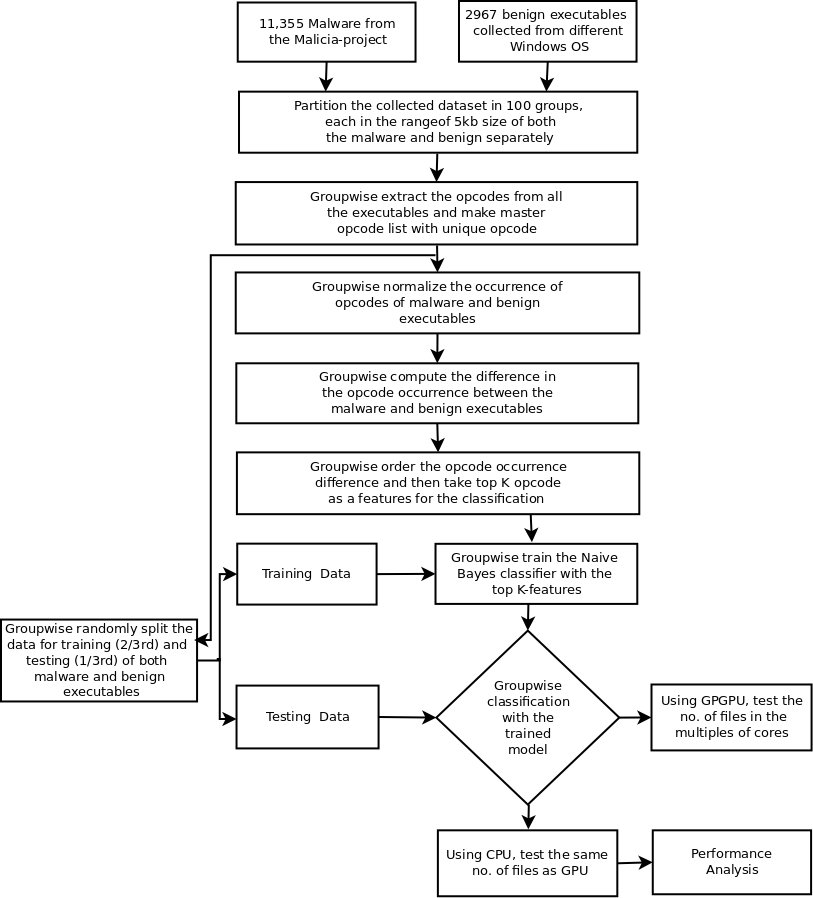
\includegraphics[scale=.24]{graphs/new1/FlowChart.png}
	\caption{Flow chart for malware detection system}
\end{figure}

Training is performed on CPU to generate the trained model by exploiting the term independence principle of Naive Bayes and malware mean, malware variance, benign mean, benign variance per group are calculated. After the completion of training we are left with the trained model and a Feature matrix representing the top K features from each group where K is given by user at the time of training. These matrices are dumped to files after the completion of training and used again testing step. 

During testing step the trained model and feature matrix are loaded in memory and represented in the form of matrices and the testing data set is also read simultaneously. The test dataset is again divided into 5KB size similar to training step [10]. Finally, all the data is loaded in GPU DRAM and Naive Bayes algorithm is applied to calculate probabilities of testing samples for assigning class label to it. The testing sample is only tested against the group corresponding to its size. This is done in order to increase the accuracy as discussed by authors in their previous findings [10].  In this whole process we used a task parallel approach for parallel implementation of detection algorithm on GPU.

\subsection{Results}    

It was observed that the parallel implementation on GPU of Naive Bayes algorithm was able to achieve an execution time performance of 45x to 52x in case of first configuration and an execution time performance boost of 100x to 125x over sequential implementation on CPU with second configuration. It was also observed that the performance gain is dependent on no of features (K) taken and the no of cores in GPU. We observed that initially the CPU execution time dominates the GPU execution time in terms of execution time performance but as soon as the no of files increases and reach a threshold the GPU dominates the CPU in terms of performance. This was because of underutilization of GPU cores due to lack of task to perform as it processes tasks in blocks and some cores were idle while CPU executes tasks one by one basis. 

In our experiment we found that the dataset size was not sufficient to observe the GPU execution time as after taking out training data we were left with 4500 samples only for testing. So, for measuring the relation between CPU and GPU execution time we considered whole dataset. Although accuracy was calculated using a split of 67\% for training and 33\% for testing. We also observed that there is always a trade-of between accuracy and execution time. The accuracy significantly decreases when the no of features (K) reduces below 90 in our dataset and after increasing K beyond 200 the accuracy does not change, best case being above 87\%. Although for smaller data set the shared memory can also be utilized. 

\begin{figure}[H]
	\centering
	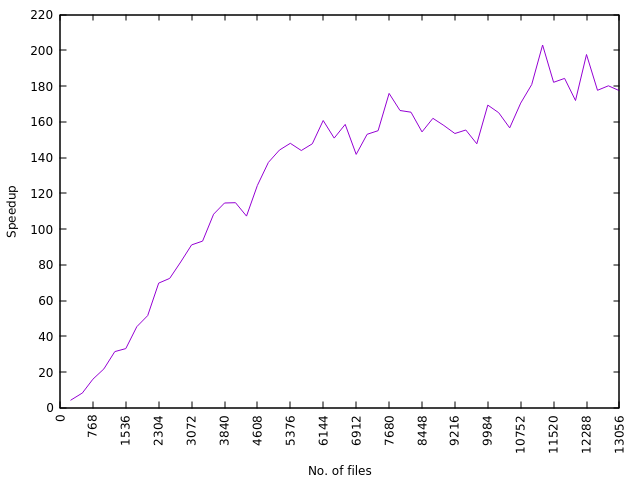
\includegraphics[scale=.5]{graphs/new1/speedup.png}
	\caption{CPU v/s GPU execution time comparison using configuration 1 using all files}
	\end{figure}
		
It was also observed that the speedup is also dependent on he number of features used for malware detection. The speedup decreases with increasing number of features for given number of cores. In our experiment we experimented with various sets of features and found that the accuracy increases with increasing the value of K (top K features) till 200, after which there is no significant change in accuracy. This situation creates a new challenge of coming up with a new and efficient feature selection technique so that the time and accuracy trade-of can be minimized.  

\begin{figure}[H]
	\centering
	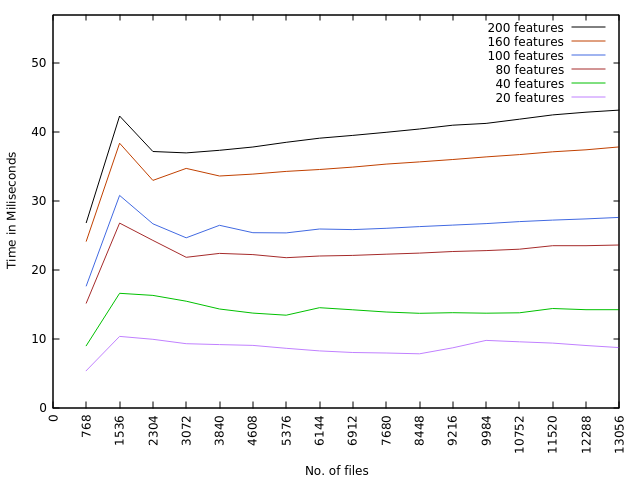
\includegraphics[scale=.5]{graphs/new1/CPU_time.png}
	\caption{CPU execution time with different number of features with configuration 2}
\end{figure}

\begin{figure}[H]
	\centering
	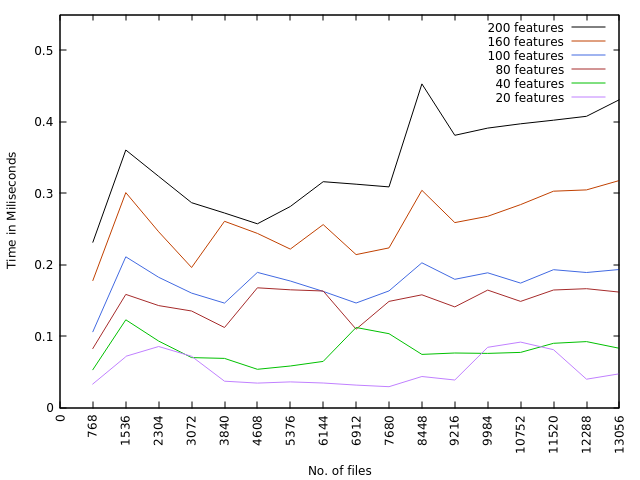
\includegraphics[scale=.5]{graphs/new1/GPU_time.png}
	\caption{GPU execution time with different number of features with configuration 2}
\end{figure}


%\begin{figure}[H]
%	\centering
%	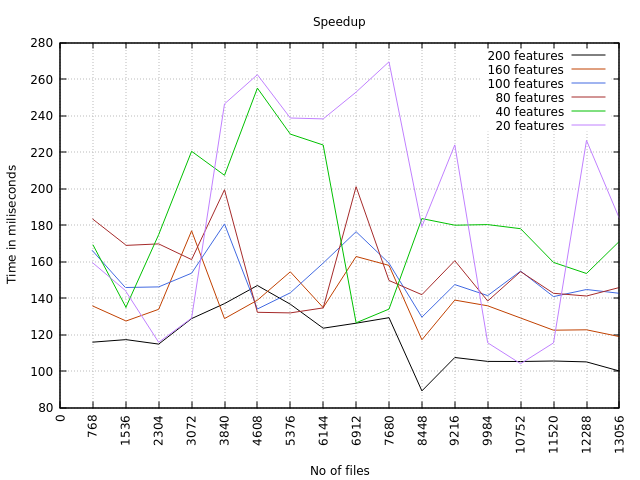
\includegraphics[scale=.5]{graphs/new/speedup.png}
%	\caption{Speedup with different number of features with configuration 2}
%\end{figure}


% An example of a floating figure using the graphicx package.
% Note that \label must occur AFTER (or within) \caption.
% For figures, \caption should occur after the \includegraphics.
% Note that IEEEtran v1.7 and later has special internal code that
% is designed to preserve the operation of \label within \caption
% even when the captionsoff option is in effect. However, because
% of issues like this, it may be the safest practice to put all your
% \label just after \caption rather than within \caption{}.
%
% Reminder: the "draftcls" or "draftclsnofoot", not "draft", class
% option should be used if it is desired that the figures are to be
% displayed while in draft mode.
%
%\begin{figure}[!t]
%\centering
%\includegraphics[width=2.5in]{myfigure}
% where an .eps filename suffix will be assumed under latex, 
% and a .pdf suffix will be assumed for pdflatex; or what has been declared
% via \DeclareGraphicsExtensions.
%\caption{Simulation Results.}
%\label{fig_sim}
%\end{figure}

% Note that IEEE typically puts floats only at the top, even when this
% results in a large percentage of a column being occupied by floats.
% However, the Computer Society has been known to put floats at the bottom.


% An example of a double column floating figure using two subfigures.
% (The subfig.sty package must be loaded for this to work.)
% The subfigure \label commands are set within each subfloat command,
% and the \label for the overall figure must come after \caption.
% \hfil is used as a separator to get equal spacing.
% Watch out that the combined width of all the subfigures on a 
% line do not exceed the text width or a line break will occur.
%
%\begin{figure*}[!t]
%\centering
%\subfloat[Case I]{\includegraphics[width=2.5in]{box}%
%\label{fig_first_case}}
%\hfil
%\subfloat[Case II]{\includegraphics[width=2.5in]{box}%
%\label{fig_second_case}}
%\caption{Simulation results.}
%\label{fig_sim}
%\end{figure*}
%
% Note that often IEEE papers with subfigures do not employ subfigure
% captions (using the optional argument to \subfloat[]), but instead will
% reference/describe all of them (a), (b), etc., within the main caption.


% An example of a floating table. Note that, for IEEE style tables, the 
% \caption command should come BEFORE the table. Table text will default to
% \footnotesize as IEEE normally uses this smaller font for tables.
% The \label must come after \caption as always.
%
%\begin{table}[!t]
%% increase table row spacing, adjust to taste
%\renewcommand{\arraystretch}{1.3}
% if using array.sty, it might be a good idea to tweak the value of
% \extrarowheight as needed to properly center the text within the cells
%\caption{An Example of a Table}
%\label{table_example}
%\centering
%% Some packages, such as MDW tools, offer better commands for making tables
%% than the plain LaTeX2e tabular which is used here.
%\begin{tabular}{|c||c|}
%\hline
%One & Two\\
%\hline
%Three & Four\\
%\hline
%\end{tabular}
%\end{table}


% Note that IEEE does not put floats in the very first column - or typically
% anywhere on the first page for that matter. Also, in-text middle ("here")
% positioning is not used. Most IEEE journals use top floats exclusively.
% However, Computer Society journals sometimes do use bottom floats - bear
% this in mind when choosing appropriate optional arguments for the
% figure/table environments.
% Note that, LaTeX2e, unlike IEEE journals, places footnotes above bottom
% floats. This can be corrected via the \fnbelowfloat command of the
% stfloats package.



\section{Conclusion}
In this work we implement parallel implementation of Naive Bayes algorithm for fast detection of malware on GPU along with size-based partitioning of malware samples for better accuracy.  In our approach we discuss a task parallel approach for parallelizing Naive Bayes classifier. We experimentally evaluated the proposed approach against the sequential version of algorithm and got a speedup of   45x to 52x with first configuration and 100x to 125x with second configuration maintaining same accuracy.  As our future work we would like to explore suitability of other parallel implementation classification algorithms and compare with our approach.  





% if have a single appendix:
%\appendix[Proof of the Zonklar Equations]
% or
%\appendix  % for no appendix heading
% do not use \section anymore after \appendix, only \section*
% is possibly needed

% use appendices with more than one appendix
% then use \section to start each appendix
% you must declare a \section before using any
% \subsection or using \label (\appendices by itself
% starts a section numbered zero.)
%


%\appendices
%\section{Proof of the First Zonklar Equation}
%Appendix one text goes here.

% you can choose not to have a title for an appendix
% if you want by leaving the argument blank
%\section{}
%Appendix two text goes here.


% use section* for acknowledgement
\ifCLASSOPTIONcompsoc
  % The Computer Society usually uses the plural form
 % \section*{Acknowledgments}
\else
  % regular IEEE prefers the singular form
%  \section*{Acknowledgment}
\fi


%The authors would like to thank...


% Can use something like this to put references on a page
% by themselves when using endfloat and the captionsoff option.
\ifCLASSOPTIONcaptionsoff
  \newpage
\fi



\bibliographystyle{ieeetr}
\bibliography{references}{}
 

% trigger a \newpage just before the given reference
% number - used to balance the columns on the last page
% adjust value as needed - may need to be readjusted if
% the document is modified later
%\IEEEtriggeratref{8}
% The "triggered" command can be changed if desired:
%\IEEEtriggercmd{\enlargethispage{-5in}}

% references section

% can use a bibliography generated by BibTeX as a .bbl file
% BibTeX documentation can be easily obtained at:
% http://www.ctan.org/tex-archive/biblio/bibtex/contrib/doc/
% The IEEEtran BibTeX style support page is at:
% http://www.michaelshell.org/tex/ieeetran/bibtex/
%\bibliographystyle{IEEEtran}
% argument is your BibTeX string definitions and bibliography database(s)
%\bibliography{IEEEabrv,../bib/paper}
%
% <OR> manually copy in the resultant .bbl file
% set second argument of \begin to the number of references
% (used to reserve space for the reference number labels box)


% biography section
% 
% If you have an EPS/PDF photo (graphicx package needed) extra braces are
% needed around the contents of the optional argument to biography to prevent
% the LaTeX parser from getting confused when it sees the complicated
% \includegraphics command within an optional argument. (You could create
% your own custom macro containing the \includegraphics command to make things
% simpler here.)
%\begin{IEEEbiography}[{\includegraphics[width=1in,height=1.25in,clip,keepaspectratio]{mshell}}]{Michael Shell}
% or if you just want to reserve a space for a photo:

%\begin{IEEEbiography}{Michael Shell}
%Biography text here.
%\end{IEEEbiography}

% if you will not have a photo at all:
%\begin{IEEEbiographynophoto}{John Doe}
%Biography text here.
%\end{IEEEbiographynophoto}

% insert where needed to balance the two columns on the last page with
% biographies
%\newpage

%\begin{IEEEbiographynophoto}{Jane Doe}
%Biography text here.
%\end{IEEEbiographynophoto}

% You can push biographies down or up by placing
% a \vfill before or after them. The appropriate
% use of \vfill depends on what kind of text is
% on the last page and whether or not the columns
% are being equalized.

%\vfill

% Can be used to pull up biographies so that the bottom of the last one
% is flush with the other column.
%\enlargethispage{-5in}



% that's all folks
\end{document}


